\section{Combinational Logic}

  Talk about how to construct arithmetic operations with these gates such as adding two integers or multiplying them, and not just that, but other operations that we may need in a programming language. 

\subsection{Multi-Bit Gates}

  Note that we can naturally work with multiple bits. This could mean a few things for---say, an AND gate. 
  \begin{enumerate}
    \item AND can take in multiple gates. 
    \item 
  \end{enumerate}

  \begin{definition}[Multi-Bit NOT Gate]
    
  \end{definition}

  \begin{definition}[Multi-Bit AND Gate]
    
  \end{definition}

  \begin{definition}[Multi-Bit OR Gate]
    
  \end{definition}

  \begin{definition}[Multi-Bit NAND Gate]
    
  \end{definition}

  \begin{definition}[Multi-Bit XOR Gate]
    
  \end{definition}

  \begin{definition}[Multi-Bit Multiplexor Gate]
    
  \end{definition}

  \begin{definition}[Multi-Bit Demultiplexor Gate]
    
  \end{definition}

\subsection{Multiplexer}

  Multiplexors are good for conditionals and implementing hierarchical functions. 

  \begin{definition}[Multiplexer]
    A \textbf{$2^n : 1$ multiplexer} is a gate that takes in 
    \begin{enumerate}
      \item $n$ \textbf{control bits} as inputs, denoted $s = (s_0, \ldots, s_n)$. 
      \item $2^n$ \textbf{input channels}, denoted $x_{s}$ for $s \in \{0, 1\}^n$. 
    \end{enumerate}
    and outputs the designated input channel according to $s$. 
    \begin{equation}
      y(s, x) = x_s
    \end{equation}

    \begin{figure}[H]
      \centering 
      \begin{tikzpicture}[circuit logic US, yscale=0.5]
        \node[muxdemux] {};
      \end{tikzpicture}
      \caption{General diagram of a multiplexer with $n=3$ control bits, $2^n = 8$ input channels, and 1 output channel.} 
    \end{figure}
  \end{definition}

  \begin{theorem}[Implementation of 2:1 Multiplexer]
    \begin{figure}[H]
      \centering 
      \begin{tikzpicture}[circuit logic US]
        \node[not gate, point down, scale=0.8] (not) at (0, 2) {}; 
        \node[and gate] (and1) at (2, 1) {}; 
        \node[and gate] (and2) at (2, 0) {}; 
        \node[or gate] (or) at (3.5, 0.5) {};

        \draw (-1, 0.9) node[left] {$w_1$} -- (and1.input 2);
        \draw (-1, -0.1) node[left] {$w_2$} -- (and2.input 2);

        \draw (and1.output) -- ++ (0.2, 0) -- ++(0, -0.4) -- (or.input 1); 
        \draw (and2.output) -- ++ (0.2, 0) -- ++(0, 0.4) -- (or.input 2); 
        \draw (0, 3) node[above] {$s$} -- (not.input); 
        \draw (not.output) -- (0, 1.1) -- (and1.input 1); 
        \draw (0, 2.5) -- (-0.5, 2.5) -- (-0.5, 0.1) -- (and2.input 1); 

        \draw (or.output) -- ++(0.3, 0) node[right] {$y$};
      \end{tikzpicture}
      \caption{The truth table grows exponentially large with $n$ and does not provide much value, so it is omitted here.} 
    \end{figure}
  \end{theorem}

  \begin{theorem}[Implementation of 4:1 Multiplexer]
    \begin{figure}[H]
      \centering 
      \begin{tikzpicture}[circuit logic US]
        % NOT gates for select lines (inverted S0 and S1)
        \node (s0) at (1, 9) {$s_0$};
        \node (s1) at (2, 9) {$s_1$};
        \node[not gate, point down, scale=0.8] (not_s0) at (3, 7.5) {}; 
        \node[not gate, point down, scale=0.8] (not_s1) at (4, 7.5) {}; 
       
        % AND gates for each input combination
        \node[and gate, inputs=nnn] (and_a3) at (6, 6.5) {};
        \node[and gate, inputs=nnn] (and_a2) at (6, 5) {}; 
        \node[and gate, inputs=nnn] (and_a1) at (6, 3.5) {};
        \node[and gate, inputs=nnn] (and_a0) at (6, 2) {}; 
       
        % OR gate for final output
        \node[or gate, inputs=nnnn] (or_out) at (9, 4.25) {};

        \draw (s0.south) -- (1, 3.5) -- (and_a1.input 2);
        \draw (s1.south) -- (2, 5.15) -- (and_a2.input 1);
        \draw (s0.south) -- ++(0, -0.7) -- ++(2, 0) -- (not_s0.west); 
        \draw (s1.south) -- ++(0, -0.5) -- ++(2, 0) -- (not_s1.west); 
        \draw (not_s0.east) -- (3, 2) -- (and_a0.input 2);
        \draw (not_s1.east) -- (4, 2.15) -- (and_a0.input 1);
        \draw (4, 3.65) -- (and_a1.input 1); 
        \draw (3, 5) -- (and_a2.input 2); 
        \draw (1, 6.5) -- (and_a3.input 2);
        \draw (2, 6.65) -- (and_a3.input 1);
       
        % Input labels and connections
        \draw (0, 6.35) node[left] {$w_3$} -- (and_a3.input 3);
        \draw (0, 4.85) node[left] {$w_2$} -- (and_a2.input 3);
        \draw (0, 3.35) node[left] {$w_1$} -- (and_a1.input 3);
        \draw (0, 1.85) node[left] {$w_0$} -- (and_a0.input 3);
       
        % Connect AND gates to OR gate
        \draw (and_a3.output) -- (7.5, 6.5) -- (7.5, 4.5) -- (or_out.input 1);
        \draw (and_a2.output) -- (7.2, 5) -- (7.2, 4.33) -- (or_out.input 2);
        \draw (and_a1.output) -- (7.2, 3.5) -- (7.2, 4.17) -- (or_out.input 3);
        \draw (and_a0.output) -- (7.5, 2) -- (7.5, 4.00) -- (or_out.input 4);

        \fill (1, 6.5) circle (1.5pt); 
        \fill (2, 6.65) circle (1.5pt); 
        \fill (3, 5) circle (1.5pt); 
        \fill (4, 3.65) circle (1.5pt); 
       
        % Output
        \draw (or_out.output) -- ++(0.5, 0) node[right] {$y$};
      \end{tikzpicture}
      \caption{Implementation of 4:1 multiplexer.}
    \end{figure}
  \end{theorem}

  There is a general method to build larger multiplexers, and so implementing for $n$ control bits is easy. Consider the simpler diagram for a 4:1 multiplexer. 

  \begin{figure}[H]
    \centering 
    \begin{tikzpicture}[circuit logic US]
      % Top multiplexer

      \node (s1) at (-1, 4) {$s_1$}; 
      \node (s0) at (-1, 3.2) {$s_0$}; 
      \node[muxdemux, muxdemux def={NL=2, Rh=4, NR=1, NT=1, NB=0, w=2}, yscale=0.4] (mux1) at (0, 1.5) {};
      \draw (mux1.lpin 1) node[left] {$w_0$};
      \draw (mux1.lpin 2) node[left] {$w_1$};
      
      % Bottom multiplexer  
      \node[muxdemux, muxdemux def={NL=2, Rh=4, NR=1, NT=1, NB=0, w=2}, yscale=0.4] (mux2) at (0, -1.5) {};
      \draw (mux2.lpin 1) node[left] {$w_2$};
      \draw (mux2.lpin 2) node[left] {$w_3$};
      
      % Right multiplexer
      \node[muxdemux, muxdemux def={NL=2, Rh=4, NR=1, NT=1, NB=0, w=2}, yscale=0.4] (mux3) at (3, 0) {};

      \draw (s1.east) -- (3, 4) -- (mux3.tpin 1); 
      \draw (s0.east) -- (0, 3.2) -- (mux1.tpin 1); 
      \draw (s0.east) -- (0, 3.2) -- ++(0, -0.5) -- ++(1, 0) -- ++(0, -3) -- ++(-1, 0) -- (mux2.tpin 1); 
      \fill (0, 2.7) circle (1.5pt);
      \draw (mux3.lpin 1) -- ++(-0.5, 0) -- ++(0, 1.05) -- (mux1.rpin 1);
      \draw (mux3.lpin 2) -- ++(-0.5, 0) -- ++(0, -1.05) -- (mux2.rpin 1);
      \node[right] at (mux3.rpin 1) {$y$};
    \end{tikzpicture}
    \caption{With this pattern, we can build arbitrarily large multiplexors.} 
  \end{figure}

\subsection{Comparator}

  \begin{definition}[1-Bit Comparator]
    A \textbf{1-bit (magnitude) comparator} simply takes in 2 1-bit numbers $a, b \in \{0, 1\}$ and outputs whether $a > b$, $a = b$, or $a < b$. 

    \begin{figure}[H]
      \centering
      \begin{subfigure}[b]{0.48\textwidth}
        \centering
        \begin{circuitikz}[circuit logic US]
          \node[op amp] (opamp) at (0, 0) {};
          \draw (opamp.+) to[short] ++(-1,0) node[left] {$b$};
          \draw (opamp.-) to[short] ++(-1,0) node[left] {$a$};
          \draw (opamp.out)++(0.5,0) -- ++(0, 0.4) -- ++(0.5, 0) node[right] {$l$};
          \draw (opamp.out) -- ++(1,0) node[right] {$e$};
          \draw (opamp.out)++(0.5,0) -- ++(0, -0.4) -- ++(0.5, 0) node[right] {$g$};
        \end{circuitikz}
        \caption{}
      \end{subfigure}
      \hfill 
      \begin{subfigure}[b]{0.48\textwidth}
        \centering
        \begin{tabular}{|c|c|c|c|c|}
          \hline
          a & b & aEQb & aGTb & bGTa \\
          \hline
          0 & 0 & 1 & 0 & 0 \\
          \hline
          0 & 1 & 0 & 0 & 1 \\
          \hline
          1 & 0 & 0 & 1 & 0 \\
          \hline
          1 & 1 & 1 & 0 & 0 \\
          \hline
        \end{tabular}
        \caption{Truth table.}
      \end{subfigure}
    \end{figure}

    The implementation is quite simple. 

    \begin{figure}[H]
      \centering 
      \begin{circuitikz}[circuit logic US, scale=1.4]
        \node[not gate, scale=0.5] (not1) at (-1.5, 1.6) {}; 
        \node[and gate] (and1) at (0, 1.5) {}; 
        \node[xnor gate] (xnor) at (0.5, 0) {}; 
        \node[and gate] (and2) at (0, -2) {}; 
        \node[not gate, point down, scale=0.5] (not2) at (-1.5, -1) {}; 
        \draw (-3.5, 1.6) node[left] {$a$} -- (not1.input);
        \draw (-3.5, 1.4) node[left] {$b$} -- (and1.input 2);
        \draw (not1.output) -- (and1.input 1);
        \draw (-2.7, 1.6) -- (-2.7, -1.9) -- (and2.input 1);
        \draw (not2.output) -- (-1.5, -2.1) -- (and2.input 2); 
        \fill (-1.5, 1.4) circle (1.5pt); 
        \fill (-1.5, -0.1) circle (1.5pt); 
        \draw (-2.7, 0.1) -- (xnor.input 1); 
        \draw (-1.5, -0.1) -- (xnor.input 2); 
        \draw (-1.5, 1.4) -- (not2.input); 
        \draw (and1.output) -- ++(0.5, 0) node[right] {$l$};
        \draw (xnor.output) -- ++(0.5, 0) node[right] {$e$};
        \draw (and2.output) -- ++(0.5, 0) node[right] {$g$};
      \end{circuitikz}
      \caption{} 
    \end{figure}
  \end{definition}

  Now that we have a 1-bit comparator, given two $n$-bit inputs, all we have to do is apply the 1-bit comparator starting from the most significant bit to the least significant bit, and this gives us an $n$-bit comparator. However, this is pretty slow since it is sequential, but implementing one-shot $n$-bit comparators requires an exponentially large circuit. Therefore, we compromise between the two schemes. The general idea is that we implement $2$-bit and $4$-bit one-shot comparators, and then use them to sequentially compare bigger---e.g. $32$-bit---numbers. 

  \begin{definition}[2-Bit Comparator]
    A 2-bit comparator is implemented as such. 

    \begin{figure}[H]
      \centering 
      \begin{circuitikz}[circuit logic US, scale=1.4]
        \foreach \w in {0, 1, 2, 3} {
          \node[not gate, scale=0.6, point down] (not) at (-4 + \w, 4) {}; 
          \draw (not.output) -- ++(0, -7); 
          \draw (-4.3 + \w, 5) -- ++(0, -8); 
          \draw (-4.3 + \w, 4.5) -- ++(0.3, 0) -- (not.input); 
          \fill (-4 + \w, 4.5) circle (1.5pt); 
        }

        \node[above] at (-4.3, 5) {$a_1$}; 
        \node[above] at (-3.3, 5) {$a_0$}; 
        \node[above] at (-2.3, 5) {$b_1$}; 
        \node[above] at (-1.3, 5) {$b_0$}; 

        \node[and gate, scale=0.8, inputs=nnn] (and1) at (1, 2 + 0.6) {}; 
        \node[and gate, scale=0.8, inputs=nnn] (and2) at (1, 2) {}; 
        \node[and gate, scale=0.8, inputs=nnn] (and3) at (1, 2 - 0.6) {}; 
        \node[nor gate, scale=0.8, inputs=nnn] (nor1) at (2, 2) {}; 
        \draw (and1.output) -- ++(0.3, 0) -- ++(0, -0.5) -- (nor1.input 1);
        \draw (and2.output) -- (nor1.input 2);
        \draw (and3.output) -- ++(0.3, 0) -- ++(0, 0.5) -- (nor1.input 3);

        \node[and gate, scale=0.8, inputs=nnn] (and4) at (1, -2 + 0.6) {}; 
        \node[and gate, scale=0.8, inputs=nnn] (and5) at (1, -2) {}; 
        \node[and gate, scale=0.8, inputs=nnn] (and6) at (1, -2 - 0.6) {}; 
        \node[nor gate, scale=0.8, inputs=nnn] (nor2) at (2, -2) {}; 
        \draw (and4.output) -- ++(0.3, 0) -- ++(0, -0.5) -- (nor2.input 1);
        \draw (and5.output) -- (nor2.input 2);
        \draw (and6.output) -- ++(0.3, 0) -- ++(0, 0.5) -- (nor2.input 3);

        \draw (-3.3, 0.7 + 2) -- (and1.input 1); 
        \draw (-2, 0.6 + 2) -- (and1.input 2); 
        \draw (-1, 0.5 + 2) -- (and1.input 3); 
        \fill (-3.3, 0.7 + 2) circle (1.5pt); 
        \fill (-2, 0.6 + 2) circle (1.5pt); 
        \fill (-1, 0.5 + 2) circle (1.5pt); 

        \draw (-4.3, 0.1 + 2) -- (and2.input 1); 
        \draw (-2, -0.1 + 2) -- (and2.input 3); 
        \fill (-4.3, 0.1 + 2) circle (1.5pt); 
        \fill (-2, -0.1 + 2) circle (1.5pt); 

        \draw (-4.3, -0.5 + 2) -- (and3.input 1); 
        \draw (-3.3, -0.6 + 2) -- (and3.input 2); 
        \draw (-1, -0.7 + 2) -- (and3.input 3); 
        \fill (-4.3, -0.5 + 2) circle (1.5pt); 
        \fill (-3.3, -0.6 + 2) circle (1.5pt); 
        \fill (-1, -0.7 + 2) circle (1.5pt); 

        \draw (-4, 0.7 - 2) -- (and4.input 1); 
        \draw (-3, 0.6 - 2) -- (and4.input 2); 
        \fill (-4, 0.7 - 2) circle (1.5pt); 
        \fill (-3, 0.6 - 2) circle (1.5pt); 

        \draw (-3, 0.1 - 2) -- (and5.input 1); 
        \draw (-2.3, - 2) -- (and5.input 2); 
        \draw (-1.3, -0.1 - 2) -- (and5.input 3); 
        \fill (-3, 0.1 - 2) circle (1.5pt); 
        \fill (-2.3, - 2) circle (1.5pt); 
        \fill (-1.3, -0.1 - 2) circle (1.5pt); 

        \draw (-4, -0.5 - 2) -- (and6.input 1); 
        \draw (-2.3, -0.7 - 2) -- (and6.input 3); 
        \fill (-4, -0.5 - 2) circle (1.5pt); 
        \fill (-2.3, -0.7 - 2) circle (1.5pt); 

        \node[xnor gate, scale=0.8, inputs=nnn] (xnor1) at (1, 0.5) {}; 
        \node[and gate, scale=0.8, inputs=nnn] (and) at (2.5, 0) {}; 
        \node[xnor gate, scale=0.8, inputs=nnn] (xnor2) at (1, -0.5) {}; 
        \draw (xnor1.output) -- ++(0.2, 0) -- ++(0, -0.4) -- (and.input 1); 
        \draw (xnor2.output) -- ++(0.2, 0) -- ++(0, 0.4) -- (and.input 3); 
        \draw (-3.3, 0.6) -- (xnor1.input 1); 
        \draw (-1.3, 0.4) -- (xnor1.input 2); 
        \draw (-4.3, -0.4) -- (xnor2.input 1); 
        \draw (-2.3, -0.6) -- (xnor2.input 2); 
        \fill (-3.3, 0.6) circle (1.5pt);
        \fill (-1.3, 0.4)  circle (1.5pt);
        \fill (-4.3, -0.4) circle (1.5pt);
        \fill (-2.3, -0.6) circle (1.5pt);

        \draw (nor1.output) -- ++(0.3, 0) node[right] {$a > b$}; 
        \draw (and.output) -- ++(0.3, 0) node[right] {$a = b$}; 
        \draw (nor2.output) -- ++(0.3, 0) node[right] {$a < b$}; 
      \end{circuitikz}
      \caption{Credits to GeeksForGeeks.} 
    \end{figure}
  \end{definition}

  \begin{definition}[4-Bit Comparator]
    A 4-bit comparator is implemented as such. 

    \begin{figure}[H]
      \centering 
      \begin{circuitikz}[circuit logic US, scale=1.4]
        \foreach \h in {0, 2, 4, 6} {
          \node[not gate, scale=0.6] (not1\h) at (-3, 0.5 + \h) {}; 
          \node[not gate, scale=0.6] (not2\h) at (-3, -0.5 + \h) {}; 
          \node[and gate, scale=0.8] (and1\h) at (-1.5, 0.4 + \h) {}; 
          \node[and gate, scale=0.8] (and2\h) at (-1.5, -0.4 + \h) {}; 
          \node[or gate, scale=0.8] (or\h) at (0, \h) {}; 
          \draw (not1\h.input) -- ++(-1, 0); 
          \draw (not2\h.input) -- ++(-1, 0); 
          \draw (not1\h.output) -- (and1\h.input 1); 
          \draw (not2\h.output) -- (and2\h.input 2); 
          \fill (-3.7, 0.5 + \h) circle (1.5pt); 
          \fill (-3.7, -0.5 + \h) circle (1.5pt); 
          \draw (-3.7, 0.5 + \h) -- (-2.7, -0.3 + \h) -- (and2\h.input 1); 
          \draw (-3.7, -0.5 + \h) -- (-2.7, 0.3 + \h) -- (and1\h.input 2); 
          \draw (and1\h.output) -- ++(0.3, 0) -- ++(0, -0.3) -- (or\h.input 1);
          \draw (and2\h.output) -- ++(0.3, 0) -- ++(0, 0.3) -- (or\h.input 2);
        }
        \node[left] at (-4.2, 0.5 + 6) {$a_3$}; 
        \node[left] at (-4.2, -0.5 + 6) {$b_3$}; 
        \node[left] at (-4.2, 0.5 + 4) {$a_2$}; 
        \node[left] at (-4.2, -0.5 + 4) {$b_2$}; 
        \node[left] at (-4.2, 0.5 + 2) {$a_1$}; 
        \node[left] at (-4.2, -0.5 + 2) {$b_1$}; 
        \node[left] at (-4.2, 0.5 + 0) {$a_0$}; 
        \node[left] at (-4.2, -0.5 + 0) {$b_0$}; 

        \node[and gate, inputs=nnnn, scale=0.7] (and1) at (1.5, 4.5) {}; 
        \node[and gate, inputs=nnnn, scale=0.7] (and2) at (1.5, 3.7) {}; 
        \node[and gate, inputs=nnnn, scale=0.7] (and3) at (1.5, 2.5) {}; 
        \node[and gate, inputs=nnnn, scale=0.7] (and4) at (1.5, 1.7) {}; 
        \node[and gate, inputs=nnnn, scale=0.7] (and5) at (1.5, 0.5) {}; 
        \node[and gate, inputs=nnnn, scale=0.7] (and6) at (1.5, -0.3) {}; 
        \node[and gate, inputs=nnnn, scale=0.7] (and7) at (1.5, -1.15) {}; 

        \draw (0.8, 0.55 + 4) -- (and1.input 2); \fill (0.8, 0.55 + 4) circle (1.5pt);
        \draw (and14.output)++(0.3, 0) -- (and1.input 4); 

        \draw (0.8, -0.25 + 4) -- (and2.input 2); \fill (0.8, -0.25 + 4) circle (1.5pt);
        \draw (and24.output)++(0.3, 0) -- (and2.input 4); 

        \draw (0.8, 0.55 + 2) -- (and3.input 2); \fill (0.8, 0.55 + 2) circle (1.5pt);
        \draw (0.7, 0.45 + 2) -- (and3.input 3); \fill (0.7, 0.45 + 2) circle (1.5pt);
        \draw (and12.output)++(0.3, 0) -- (and3.input 4); 
        \fill (and12.output)++(0.3, 0) circle (1.5pt); 

        \draw (0.8, -0.25 + 2) -- (and4.input 2); \fill (0.8, -0.25 + 2) circle (1.5pt);
        \draw (0.7, -0.35 + 2) -- (and4.input 3); \fill (0.7, -0.35 + 2) circle (1.5pt);
        \draw (and22.output)++(0.3, 0) -- (and4.input 4); 
        \fill (and22.output)++(0.3, 0) circle (1.5pt); 

        \draw (0.8, 0.65) -- (and5.input 1); \fill (0.8, 0.65) circle (1.5pt);
        \draw (0.7, 0.55) -- (and5.input 2); \fill (0.7, 0.55) circle (1.5pt);
        \draw (0.6, 0.45) -- (and5.input 3); \fill (0.6, 0.45) circle (1.5pt);
        \draw (and10.output)++(0.3, 0) -- (and5.input 4); 
        \fill (and10.output)++(0.3, 0) circle (1.5pt); 

        \draw (0.8, -0.15) -- (and6.input 1); \fill (0.8, -0.15) circle (1.5pt);
        \draw (0.7, -0.25) -- (and6.input 2); \fill (0.7, -0.25) circle (1.5pt);
        \draw (0.6, -0.35) -- (and6.input 3); \fill (0.6, -0.35) circle (1.5pt);
        \draw (and20.output)++(0.3, 0) -- (and6.input 4); 
        \fill (and20.output)++(0.3, 0) circle (1.5pt); 

        \draw (or0.output) -- ++(0.1, 0) -- (0.5, -1.3) -- (and7.input 4); 
        \draw (or2.output) -- ++(0.2, 0) -- (0.6, -1.2) -- (and7.input 3); 
        \draw (or4.output) -- ++(0.3, 0) -- (0.7, -1.1) -- (and7.input 2); 
        \draw (or6.output) -- ++(0.4, 0) -- (0.8, -1.0) -- (and7.input 1); 

        \node[or gate, scale=0.7, inputs=nnnn] (ori) at (3.3, 2.55) {}; 
        \draw (and16.output)++(0.6, 0) -- ++(3.1, 0) -- ++ (0, -3.7) -- (ori.input 1); 
        \draw (and1.output) -- ++(0.6, 0) -- ++(0, -1.9) -- (ori.input 2);
        \draw (and3.output) -- ++(0.6, 0) -- ++(0, 0) -- (ori.input 3);
        \draw (and5.output) -- ++(0.6, 0) -- ++(0, 1.9) -- (ori.input 4);

        \node[or gate, scale=0.7, inputs=nnnn] (oro) at (3, 0.1) {}; 
        \draw (and26.output)++(0.4, 0) -- ++(3, 0) -- ++ (0, -5.35) -- (oro.input 1); 
        \draw (and2.output) -- ++(0.3, 0) -- ++(0, -3.55) -- (oro.input 2);
        \draw (and4.output) -- ++(0.2, 0) -- ++(0, -1.65) -- (oro.input 3);
        \draw (and6.output) -- ++(0.2, 0) -- ++(0, 0.25) -- (oro.input 4);

        \draw (ori.output) -- ++(0.2, 0) node[right] {$a < b$}; 
        \draw (oro.output) -- ++(0.2, 0) node[right] {$a > b$}; 
        \draw (and7.output) -- ++ (1.8, 0) node[right] {$a = b$}; 
      \end{circuitikz}
      \caption{Implementation of 4-bit magnitude comparator.} 
    \end{figure}
  \end{definition}

  Therefore, 

  \begin{definition}[$n$-Bit Comparator]
    A $n$-bit comparator is implemented sequentially with 4-bit comparators. 
  \end{definition}

\subsection{Addition and Subtraction} 

  We present a hierarchy of three adders, leading to a multi-bit adder chip. Note that every single chip here represents a finite function, and so from  \hyperref[th-thm:aon_univ]{universality of AON gates} we know that an implementation is definitely possible. 
  
  \begin{definition}[Half-Adder Chip] 
    A \textbf{half-adder} is designed to add two bits. 

    \begin{figure}[H]
      \centering
      \begin{subfigure}[b]{0.48\textwidth}
        \centering
        \begin{tabular}{|c|c||c|c|}
          \hline
          \multicolumn{2}{|c||}{\textbf{Inputs}} & \multicolumn{2}{c|}{\textbf{Outputs}} \\
          \hline
          \textbf{a} & \textbf{b} & \textbf{carry} & \textbf{sum} \\
          \hline
          0 & 0 & 0 & 0 \\
          \hline
          0 & 1 & 0 & 1 \\
          \hline
          1 & 0 & 0 & 1 \\
          \hline
          1 & 1 & 1 & 0 \\
          \hline
        \end{tabular}
        \caption{Truth table for half adder.}
      \end{subfigure}
      \hfill 
      \begin{subfigure}[b]{0.48\textwidth}
        \centering
        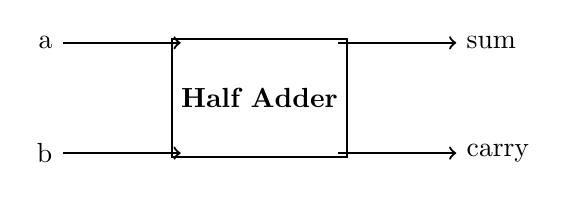
\begin{tikzpicture}
          % Block diagram
          \node[rectangle, draw, thick, minimum width=2cm, minimum height=1.5cm, font=\bfseries] 
              (halfadder) at (0, 0) {Half Adder};

          % Input lines
          \draw[thick, ->] (-2.5, 0.7) -- (-1, 0.7) node[left] at (-2.5, 0.7) {a};
          \draw[thick, ->] (-2.5, -0.7) -- (-1, -0.7) node[left] at (-2.5, -0.7) {b};

          % Output lines  
          \draw[thick, ->] (1, 0.7) -- (2.5, 0.7) node[right] at (2.5, 0.7) {sum};
          \draw[thick, ->] (1, -0.7) -- (2.5, -0.7) node[right] at (2.5, -0.7) {carry};
        \end{tikzpicture}
        \caption{}
      \end{subfigure}
      \caption{Chip diagram for half adder.}
    \end{figure}
  \end{definition}

  \begin{theorem}[Implementation of Half-Adder]
    To construct this chip, note that the way sum and carry acts on $a, b$ is identical to the standard $\XOR(a, b)$ and $\AND(a, b)$ functions. 

    \begin{figure}[H]
      \centering
      \begin{subfigure}[b]{0.48\textwidth}
        \centering
        \begin{tikzpicture}[circuit logic US]
          % Input nodes
          \node (a) at (0,2.6) {a};
          \node (b) at (0,1.4) {b};

          % Logic gates
          \node[xor gate, draw] (xor1) at (3,2.5) {};
          \node[and gate, draw] (and1) at (3,1.5) {};

          % Output labels
          \node (sum) at (5,2.5) {sum};
          \node (carry) at (5,1.5) {carry};

          % Input connections
          \draw (a) -| (xor1.input 1);
          \draw (a) -- (1, 2.6) -- (1, 1.6) -| (and1.input 1);
          \draw (b) -- (1.5, 1.4) -- (1.5, 2.4) -| (xor1.input 2);
          \draw (b) -| (and1.input 2);

          % Output connections
          \draw (xor1.output) -- (sum);
          \draw (and1.output) -- (carry);

          % Add dots at connection points for clarity
          \fill (1.5,1.4) circle (1.5pt);
          \fill (1,2.6) circle (1.5pt);
        \end{tikzpicture}
        \caption{}
      \end{subfigure}
      \hfill 
      \begin{subfigure}[b]{0.48\textwidth}
        \centering
        \begin{lstlisting}
          module half_adder(
            input a, b, 
            output s, c
          ); 
            assign s = a ^ b;
            assign c = a & b;
          endmodule
        \end{lstlisting}
        \caption{HDL implementation.}
      \end{subfigure}
      \caption{}
    \end{figure}
  \end{theorem}

  \begin{definition}[Full-Adder] 
    Now that we know how to add two bits, a \textbf{full-adder chip}  allows us to add 3 bits. 

    \begin{figure}[H]
      \centering
      \begin{subfigure}[b]{0.48\textwidth}
        \centering
        \begin{tabular}{|c|c|c||c|c|}
          \hline
          \multicolumn{3}{|c||}{\textbf{Inputs}} & \multicolumn{2}{c|}{\textbf{Outputs}} \\
          \hline
          \textbf{a} & \textbf{b} & \textbf{cin} & \textbf{cout} & \textbf{sum} \\
          \hline
          0 & 0 & 0 & 0 & 0 \\
          \hline
          0 & 0 & 1 & 0 & 1 \\
          \hline
          0 & 1 & 0 & 0 & 1 \\
          \hline
          0 & 1 & 1 & 1 & 0 \\
          \hline
          1 & 0 & 0 & 0 & 1 \\
          \hline
          1 & 0 & 1 & 1 & 0 \\
          \hline
          1 & 1 & 0 & 1 & 0 \\
          \hline
          1 & 1 & 1 & 1 & 1 \\
          \hline
        \end{tabular}
        \caption{Truth table for full adder.}
      \end{subfigure}
      \hfill 
      \begin{subfigure}[b]{0.48\textwidth}
        \centering
        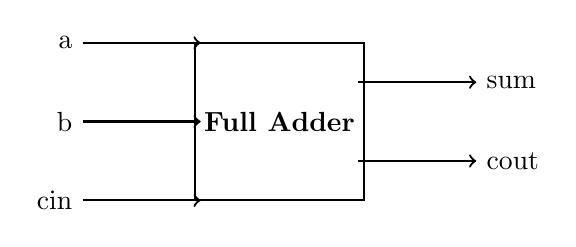
\begin{tikzpicture}
          % Block diagram
          \node[rectangle, draw, thick, minimum width=2cm, minimum height=2cm, font=\bfseries] 
              (fulladder) at (0, 0) {Full Adder};
          % Input lines
          \draw[thick, ->] (-2.5, 1) -- (-1, 1) node[left] at (-2.5, 1) {a};
          \draw[thick, ->] (-2.5, 0) -- (-1, 0) node[left] at (-2.5, 0) {b};
          \draw[thick, ->] (-2.5, -1) -- (-1, -1) node[left] at (-2.5, -1) {cin};
          % Output lines  
          \draw[thick, ->] (1, 0.5) -- (2.5, 0.5) node[right] at (2.5, 0.5) {sum};
          \draw[thick, ->] (1, -0.5) -- (2.5, -0.5) node[right] at (2.5, -0.5) {cout};
        \end{tikzpicture}
        \caption{Block diagram for full adder.}
      \end{subfigure}
      \caption{Chip diagram for full adder.}
    \end{figure}
  \end{definition}

  \begin{theorem}[Implementation of Full-Adder]
    We can implement a full adder with 2 half-adders and an $\OR$ gate. 

    \begin{figure}[H]
      \centering 
      \begin{tikzpicture}[circuit logic US]
        % Input labels
        \node at (0, 2.8) {A};
        \node at (0, 2.2) {B};
        \node at (0, 1.6) {C};

        % First Half Adder
        \node[rectangle, draw, minimum width=2cm, minimum height=1.2cm] 
          (ha1) at (2.5, 2.5) {Half Adder};

        % Second Half Adder
        \node[rectangle, draw, minimum width=2cm, minimum height=1.2cm] 
          (ha2) at (5.6, 1.9) {Half Adder};

        \node[or gate, draw, scale=1.7] (or1) at (8, 2.5) {};

        \draw (0.2, 2.75) -- (1.5, 2.75);
        \draw (0.2, 2.25) -- (1.5, 2.25);
        \draw (0.2, 1.6) -- (4.6, 1.6);

        \draw (3.5, 2.75) -| (or1.input 1);
        \draw (3.5, 2.25) -- (4.6, 2.25);
        \draw (6.6, 2.25) -| (or1.input 2);
        \draw (or1.output) |- (9.4, 2.5);
        \draw (6.6, 1.6) -- (9.4, 1.6);
        \node at (9.8, 2.5) {Carry};
        \node at (9.8, 1.6) {Sum};
      \end{tikzpicture}
      \caption{} 
    \end{figure}
  \end{theorem}

  \begin{definition}[N-Bit Adder]
    Usually, $N$ is $16, 32, 64$, or $128$. 
  \end{definition}

  \begin{theorem}[Implementation of $N$-Bit Addition]

    \begin{figure}[H]
      \centering 
      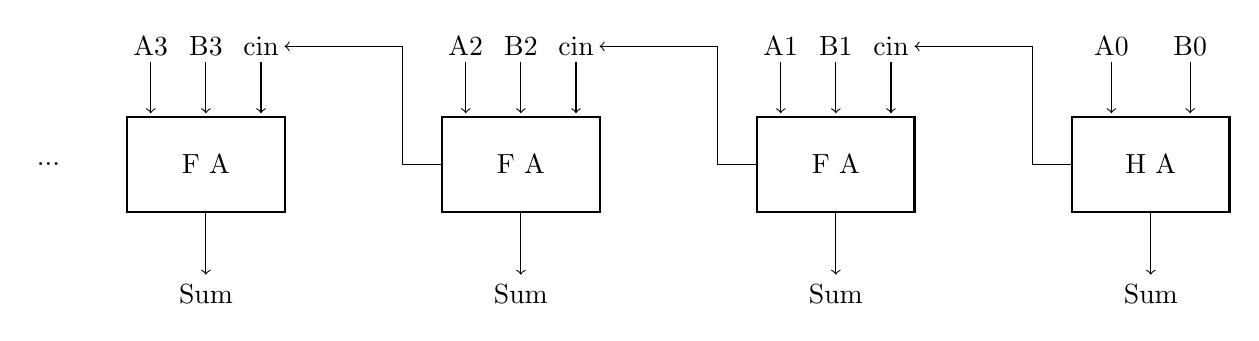
\begin{tikzpicture}
        % Input labels at the top
        \node at (1.3, 5) {A3};
        \node at (2, 5) {B3};
        \node at (2.7, 5) {cin};
        \draw[->] (1.3, 4.8) -- (1.3, 4.15);
        \draw[->] (2, 4.8) -- (2, 4.15);
        \draw[->] (2.7, 4.8) -- (2.7, 4.15);

        \node at (5.3, 5) {A2};
        \node at (6, 5) {B2};
        \node at (6.7, 5) {cin};
        \draw[->] (5.3, 4.8) -- (5.3, 4.15);
        \draw[->] (6, 4.8) -- (6, 4.15);
        \draw[->] (6.7, 4.8) -- (6.7, 4.15);

        \node at (9.3, 5) {A1};
        \node at (10, 5) {B1};
        \node at (10.7, 5) {cin};
        \draw[->] (9.3, 4.8) -- (9.3, 4.15);
        \draw[->] (10, 4.8) -- (10, 4.15);
        \draw[->] (10.7, 4.8) -- (10.7, 4.15);

        \node at (13.5, 5) {A0};
        \node at (14.5, 5) {B0};
        \draw[->] (13.5, 4.8) -- (13.5, 4.15);
        \draw[->] (14.5, 4.8) -- (14.5, 4.15);

        \node[rectangle, draw, thick, minimum width=2cm, minimum height=1.2cm] 
          (fa3) at (2, 3.5) {F A};
        \node[rectangle, draw, thick, minimum width=2cm, minimum height=1.2cm] 
          (fa2) at (6, 3.5) {F A};
        \node[rectangle, draw, thick, minimum width=2cm, minimum height=1.2cm] 
          (fa1) at (10, 3.5) {F A};
        \node[rectangle, draw, thick, minimum width=2cm, minimum height=1.2cm] 
          (ha0) at (14, 3.5) {H A};

        \draw[->] (2, 2.9) -- (2, 2.1);
        \node[below] at (2, 2.1) {Sum};

        \draw[->] (6, 2.9) -- (6, 2.1);
        \node[below] at (6, 2.1) {Sum};

        \draw[->] (10, 2.9) -- (10, 2.1);
        \node[below] at (10, 2.1) {Sum};

        \draw[->] (14, 2.9) -- (14, 2.1);
        \node[below] at (14, 2.1) {Sum};

        \draw[->] (13,3.5) -- (12.5, 3.5) -- (12.5, 5) -- (11, 5);
        \draw[->] (9,3.5) -- (8.5, 3.5) -- (8.5, 5) -- (7, 5);
        \draw[->] (5,3.5) -- (4.5, 3.5) -- (4.5, 5) -- (3, 5);
        \node at (0, 3.5) {...};
      \end{tikzpicture}
      \caption{Ripple carry adder for the last 4 significant bits of two $N$-bit numbers.} 
    \end{figure}
  \end{theorem}

  \begin{corollary}[Implemention for $N$-Bit Subtraction]
    
  \end{corollary}

  This is a standard construction and a goods start, but there are a few pitfalls of this. First, this does not detect nor handle overflows after adding. This will be handled at the operating system level. Second, addition is limited in that we can only apply it for precisely 2 arguments. 

  Ripple carry, carry select, carry look ahead adder to make it parallel (lecture 4)

  \begin{example}[More Arguments for Binary Addition]
    Note that the full adder---which takes in 3 bits---was designed so that there is enough space for each digit of the 2 inputs, plus a potential carry. If there were 3 inputs, then the full adder would need to support 4 inputs. Even worse, if we have $1 + 1 + 1 + 1 = 100$, then our carry digit will be greater than 1 digit, which messes things up even more. 
  \end{example}

  Finally, note that this is not a very efficient way to add because there are delays as the carry bit propagates from the least significant to the most significant bit pair. We can improve this with carry look-ahead techniques. 


\subsection{Multiplication} 

  Booths algo to do multiplication fast with bitshifts and addition 

  The reason bitshift is introduced first is that in binary, bit-shifting is equivalent to multiplication! 

  \begin{theorem}[Implementation of Multiplication in Circuits]
    
  \end{theorem}

  \begin{theorem}[Implementation of Moving Data in Circuits]
    
  \end{theorem}

\subsection{Arithmetic Logical Unit (ALU)}

\subsection{Control Unit} 

  The CPU also has a \textbf{control unit}, which is responsible for fetching instructions from memory through the \textbf{databus}, which is literally a wire connecting the CPU and RAM, and executing them. 

